\documentclass[a4paper,10pt]{article}
\usepackage{Sweave}
\begin{document}
\Sconcordance{concordance:PreReport.tex:PreReport.Rnw:%
1 7 1 1 0 7 1 1 5 10 1 1 6 1 0 4 1 3 0 1 2 10 1 1 2 16 0 1 2 1 4 3 1 1 %
10 2 0 1 2 4 0 1 5 9 1 1 6 1 0 3 1 3 0 1 5 29 1 1 5 1 3 2 0 2 1 5 0 1 1 %
5 0 1 1 5 0 1 1 6 0 1 2 1 4 15 1 1 7 1 0 3 1 1 2 4 0 1 2 10 1 1 2 1 0 1 %
1 1 2 6 0 1 2 6 0 1 2 13 0 1 5 7 1 1 2 1 0 3 1 6 0 1 2 4 1 1 2 1 0 1 1 %
5 0 1 1 6 0 1 2 1 1 1 2 1 0 1 1 1 2 1 0 1 1 6 0 1 2 1 1 1 70 27 1 1 6 1 %
4 3 0 1 1 3 0 1 2 1 4 15 1 11 0 1 10 3 1 11 0 1 10 2 1 24 0 1 23 7 1 1 %
6 1 7 1 4 9 1 1 6 1 9 1 4 13 1 1 7 1 0 1 1 1 7 6 0 1 1 1 2 1 1 5 0 1 1 %
5 0 1 1 5 0 1 1 6 0 1 5 11 1 12 0 1 11 5 1 14 0 1 13 17 1 14 0 1 13 5 1 %
1 6 1 0 5 1 3 0 1 5 8 1 1 2 20 0 1 18 30 1 1 7 2 0 4 1 5 0 1 1 6 0 1 5 %
11 1 1 2 1 0 3 1 1 2 1 0 3 1 4 0 1 3 11 1 1 3 2 0 1 2 1 0 1 3 2 0 1 2 4 %
0 1 2 2 1 1 3 2 0 1 1 1 2 1 0 1 2 1 0 1 1 3 0 1 2 35 1}


\title{UNDIFINED}
\maketitle
\section{Introduction}
\subsection{Background}
The core graphics system in R can been divided in to two main packages. The first package is the graphics package. It is older and it provides the original GRZ graphics system from S, sometimes referred to as ``traditional'' graphics. It is relatively fast and many other R packages build on top of it. The newer package is the grid package. It is actually slower but is has more flexibility and additional features compared to the graphics package. \\
A graph that is drawn using grid can been edited in many more ways than a graph that has been drawn using the basic graphics package. However, there is a new package, called \texttt{gridGraphics}, which allows us to convert a plot that has been drawn by the \texttt{graphics} package to an equivalent plot drawn by \texttt{grid} graphics. This means that the additional flexibility and features of grid become available for any plot drawn using the \texttt{graphics} package. \\


\subsection{The \texttt{gridGraphics} package}
\texttt{gridGraphics} is like a 'translator' that translates a plot that has been drawn using the basic graphics package to a plot that has been drawn using the grid package. \\
The \texttt{gridGraphic} package has a main function called \texttt{grid.echo()}, which takes a recorded plot as an argument (or NULL for the current plot of the current graphics device). The grid.echo() replicates theplot using grid so that the user may edite the plot in more ways than they can with the original plot drawn by bacis graphic package.\\
The following code provides a quick example. We generate 25 random numbers for x and y. First, we draw a scatter plot using the function \texttt{plot()} from the basic graphics package, then we redraw it using \texttt{grid.echo()} from the \texttt{gridGraphics} package with grid.
\begin{Schunk}
\begin{Sinput}
> pdf("figure/report_basic_demo_%0d.pdf", onefile=FALSE)
> dev.control("enable")
> set.seed(110)
> x = runif(25)
> y = runif(25)
> plot(x,y, pch = 16)
> grid.echo()
\end{Sinput}
\end{Schunk}
\begin{figure}[h]
\begin{center}
  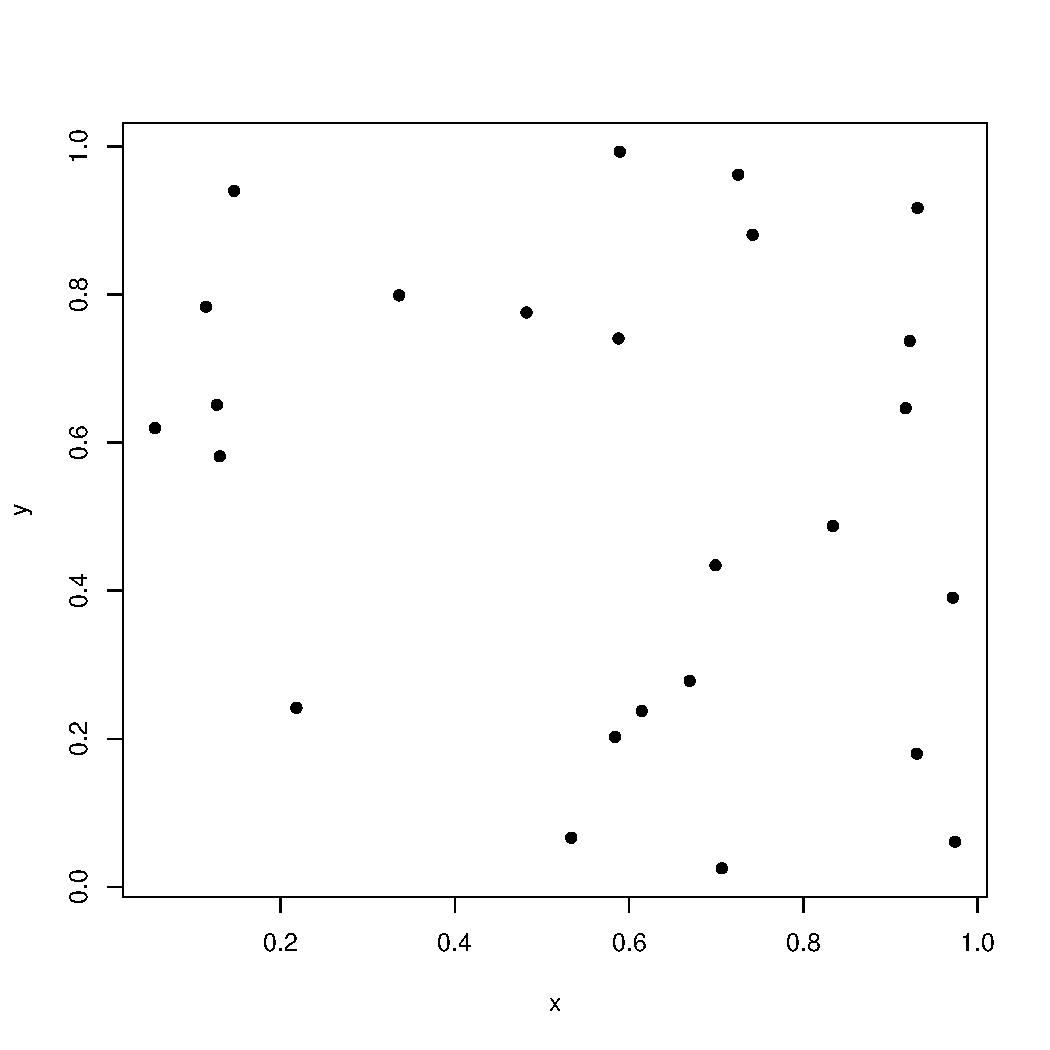
\includegraphics[height = 6cm, width = 6cm]{figure/report_basic_demo_1.pdf}
  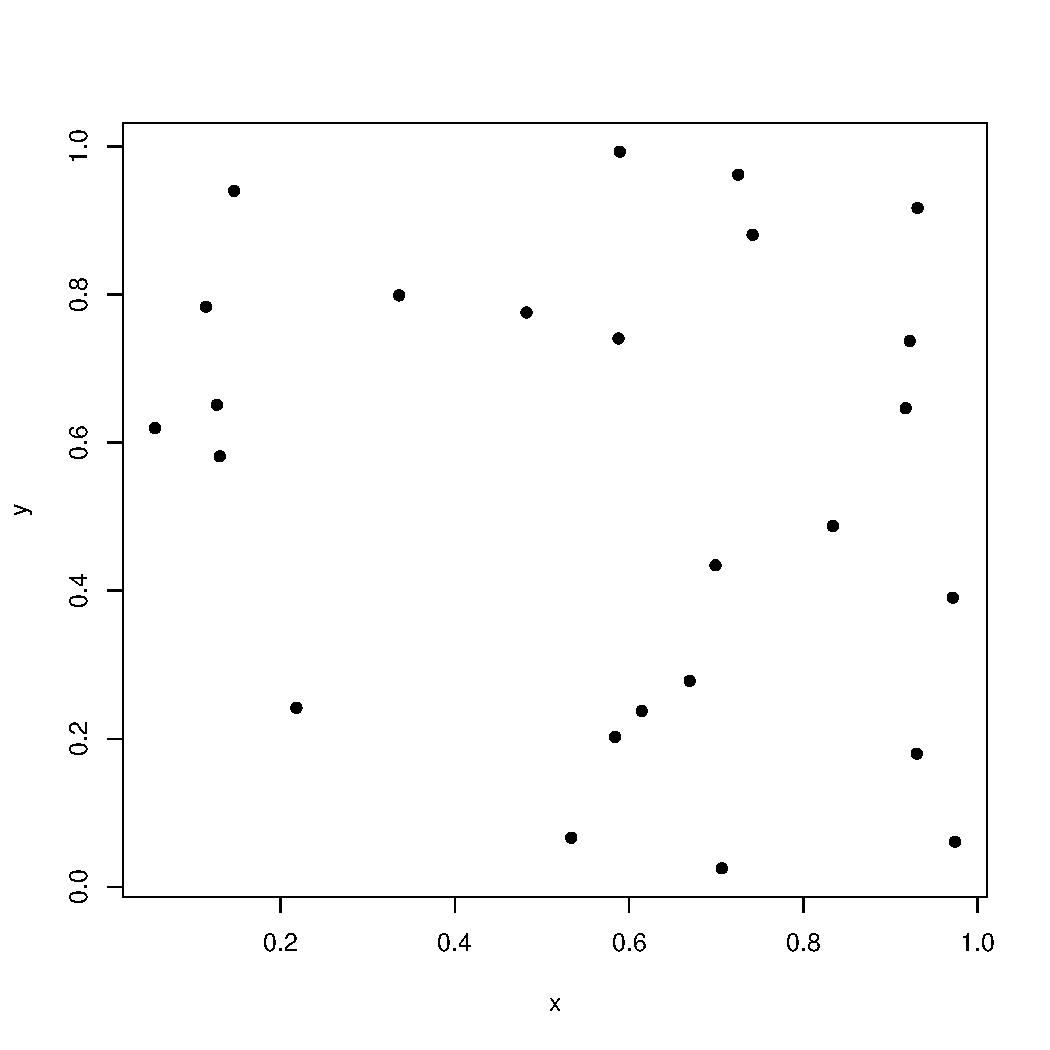
\includegraphics[height = 6cm, width = 6cm]{figure/report_basic_demo_1.pdf}
  \caption{The left plot is drawn by using plot(); the Right plot is redrawn using grid.echo(). Overall, two plots are identical to each other}
  	\label{figure1}
\end{center}
\end{figure}
One example that shows the advantage of drawing the plot using grid rather than basic graphics is that there are objects, called grid grobs, which recored a list of the details of each components of the plot that has been drawn. The list of grobs can been seen by calling the function \texttt{grid.ls()}. \\
\begin{Schunk}
\begin{Sinput}
> grid.ls()
\end{Sinput}
\begin{Soutput}
graphics-plot-1-points-1
graphics-plot-1-bottom-axis-line-1
graphics-plot-1-bottom-axis-ticks-1
graphics-plot-1-bottom-axis-labels-1
graphics-plot-1-left-axis-line-1
graphics-plot-1-left-axis-ticks-1
graphics-plot-1-left-axis-labels-1
graphics-plot-1-box-1
graphics-plot-1-xlab-1
graphics-plot-1-ylab-1
\end{Soutput}
\end{Schunk}


As we see, the \texttt{grid.ls()} function returns a list of grid grobs for the previous plot that has been redrawn by \texttt{grid}. There is one element called "graphics-plot-1-bottom-axis-labels-1" which represents the labels of the bottom axis. In \texttt{grid}, there are several functions that can be used to mainpulate this grob. For example, if the user wants to rotate the labels of the bottom axis by 30 degrees and changes the color from default to orange, then the following code performs these changes.\\


\begin{Schunk}
\begin{Sinput}
> grid.edit("graphics-plot-1-bottom-axis-labels-1", 
+           rot=30, gp=gpar(col="orange"))
> grid.edit("graphics-plot-1-left-axis-labels-1", 
+           rot=30, gp=gpar(col="orange"))
\end{Sinput}
\end{Schunk}

\begin{figure}[h]
\begin{center}
  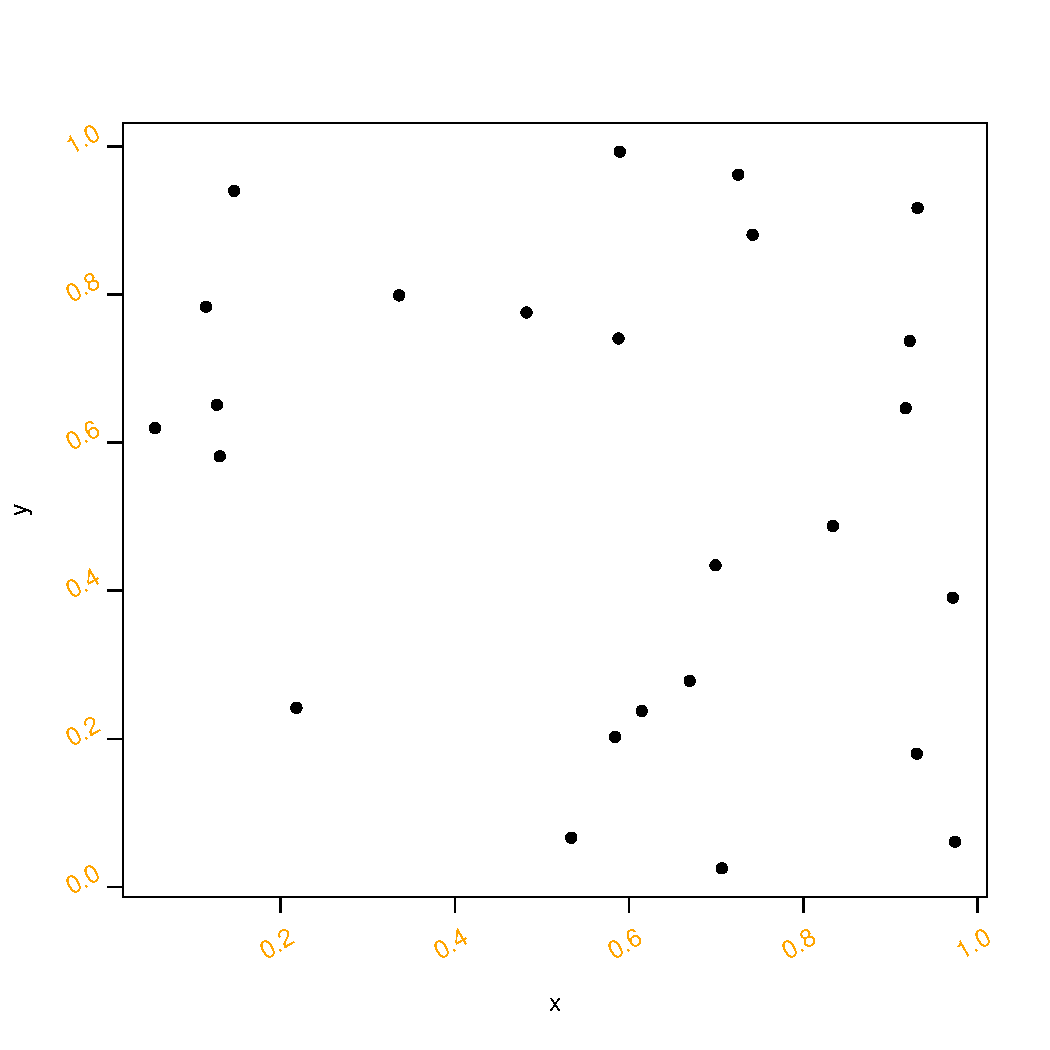
\includegraphics[height = 10cm, width = 10cm]{figure/report_basic_demo_4.pdf}
  \caption{The angle and the color of the bottom and left axis of the previous plot have been changed by 30 degrees and orange}
  	\label{figure3}
\end{center}
\end{figure}


\subsection{The problem}
The \texttt{grid.echo()} function can replicate most plots that are drawn by the graphics package. However, there are a few functions in the graphics package that \texttt{grid.echo()} cannot replicate. One such function is persp() which draws 3-dimemtional surfaces, the other one is the \texttt{filled.contour()}. If we can draw a plot with \texttt{persp()} or \texttt{filled.countour(),} the result from calling \texttt{grid.echo()} is a (mostly) blank screen. \\


\begin{Schunk}
\begin{Sinput}
> x <- y <- seq(-4*pi, 4*pi, len = 27)
> r <- sqrt(outer(x^2, y^2, "+"))
> filled.contour(cos(r^2)*exp(-r/(2*pi)), frame.plot = FALSE, plot.axes = {})
> grid.echo()
\end{Sinput}
\end{Schunk}

\begin{figure}[h]
\begin{center}
  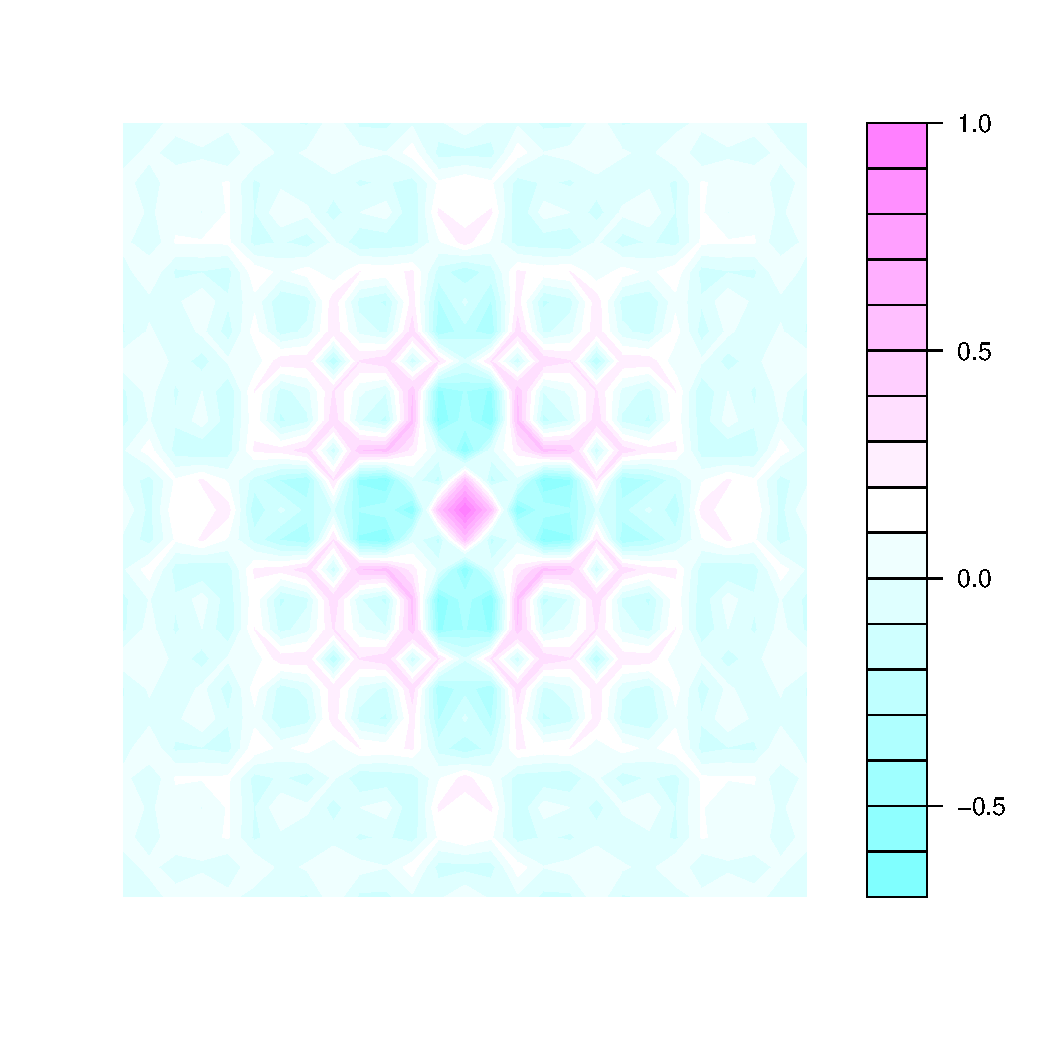
\includegraphics[height = 6cm, width = 6cm]{figure/report_fill_1}
  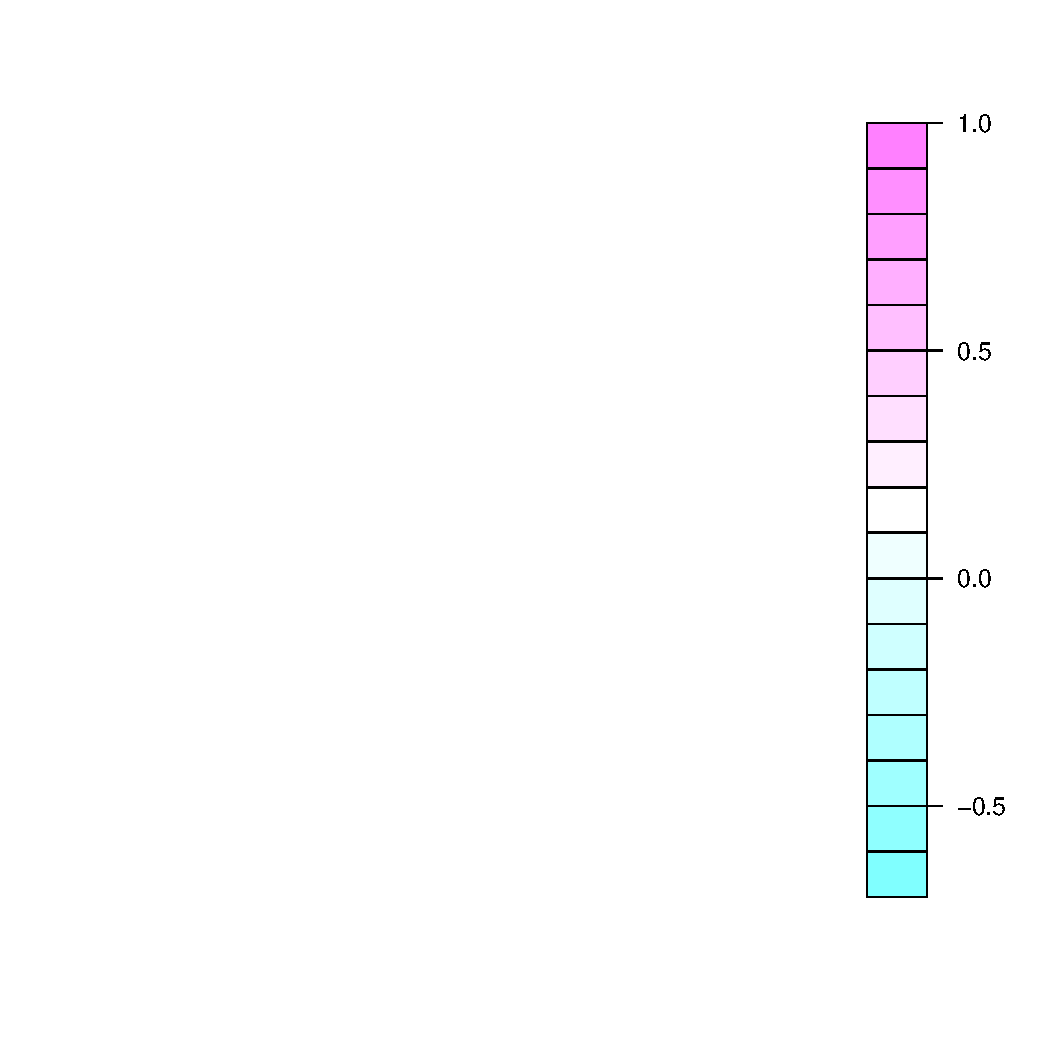
\includegraphics[height = 6cm, width = 6cm]{figure/report_fill_2}
  \caption{The left plot been drawn by using \texttt{filled.contour} and the right plot been redrawn by calling \texttt{grid.echo()}. There is a "blank" page on the right plot because the grid.echo cannot emulate filled.contour()}
  	\label{figure4}
\end{center}
\end{figure}

\newpage
\subsection{Aim of this project}
The functions \texttt{persp()} and \texttt{filled.contour()} are written in C. However, it is very hard to debug and track the C code. One possible solution will be:  \\

\begin{enumerate}
  \item emulate the \texttt{persp()} function on \texttt{grid} separate from the \texttt{gridGraphics} package (standalone):
    \begin{enumerate}
      \item Extract the information from the graphics engine display list.
      \item Understanding and translating the calculation that been done by C code from the \texttt{graphics} package to R code
      \item Draw the Perspective Plot on \texttt{grid}.
    \end{enumerate}
  \item Connect the standalone to the \texttt{gridGraphics}
\end{enumerate}

\section{comment}
NOTE to Jason: explain how gridGraphics works first: graphics display list; gridGraphics implements an R version of each low-level C function on the display list (e.g., for C\_plot\_xy there is an R function called C\_plot\_xy in the gridGraphics package). THEN maybe write about 3D to 2D transformations, but only maybe.


\section{The graphics engine display list}
The information for every plot drawn by R can be recorded. For example, In the simple \texttt{plot()} function, it is possible to obtain the parameters for x and y, even the label of the x-axis and y-axis.\\
This information is called the graphics engine display list. In this paper, we use this graphics engine display list to replicate the \texttt{persp()} plot and texttt{filled.contour()} plot using grid.\\

The \texttt{recordPlot()} function can be used to access the graphics engine display list, the \texttt{recordPlot()} function been used. This function saves the plot in an R object. 


\begin{Schunk}
\begin{Sinput}
> plot(cars$speed, cars$dist, col = 'orange', 
+       pch = 16, xlab = 'speed', ylab = 'dist')
> reco = recordPlot()
> ## Displays the inputs 
> reco[[1]][[4]][[2]][[2]]
\end{Sinput}
\begin{Soutput}
$x
 [1]  4  4  7  7  8  9 10 10 10 11 11 12 12 12 12 13 13 13 13 14 14 14 14 15 15
[26] 15 16 16 17 17 17 18 18 18 18 19 19 19 20 20 20 20 20 22 23 24 24 24 24 25

$y
 [1]   2  10   4  22  16  10  18  26  34  17  28  14  20  24  28  26  34  34  46
[20]  26  36  60  80  20  26  54  32  40  32  40  50  42  56  76  84  36  46  68
[39]  32  48  52  56  64  66  54  70  92  93 120  85

$xlab
[1] "cars$speed"

$ylab
[1] "cars$dist"
\end{Soutput}
\end{Schunk}


\begin{figure}[h]
\begin{center}
  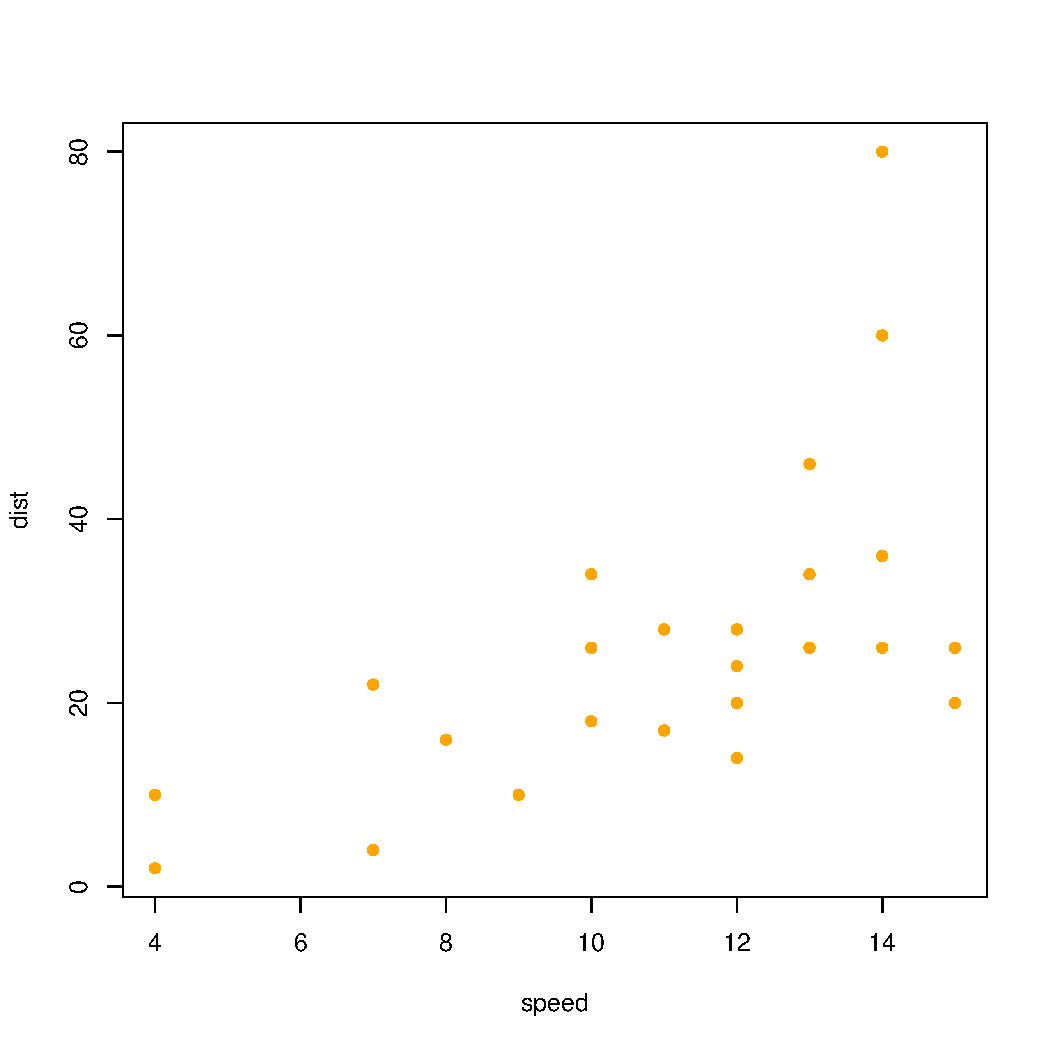
\includegraphics[height = 8cm, width = 8cm]{figure/report_3}
  \caption{dist vs speed}
  	\label{figure4}
\end{center}
\end{figure}


This example shows that: suppose we have a data set called \texttt{cars}, which contain two columns, the speed of the cars and the distance of travel. We have a plot which plotted the speed againist to the distance of travel. The \texttt{recordPlot()} will save this plot as an R object. As result, we can access the information of this plot. The last line of the code will access the x-coordinate and the y-coordinate, or the x-label and the y-label. \\

There are many way for solving this problem, one possible solution will be translate the C code to R code such that they are as simliar as possible. The reason for doing this direct translation include: \\\\
1. It is hard to debug and track the C code. \\
2. It is very simple to debug the R code. If the R code is almost identical to the C code, then we can debug the R code to ensure that the R code can also provide the same result. \\

\newpage
\section{standalone}
The Perspective Plots is used to draw a surface over the x-y plane. Usually, it has three main argument, \emph{x, y z}. \emph{x} and \emph{y} are the locations of grid line which the value z been measured, \emph{z} is a matrix which containing the values that been used to plot, or it is the matrix that been calculated by a specific function, such as 3-D mathematical functions. The following example shows how to draw a obligatory mathematical surface rotated sinc function on Perspective Plot.\\


\begin{Schunk}
\begin{Sinput}
> x = y = seq(-10, 10, length= 30)
> f <- function(x, y) { r <- sqrt(x^2+y^2); 10 * sin(r)/r }
> z <- outer(x, y, f)
> z[is.na(z)] <- 1
> trans = persp(x, y, z, theta = 30, phi = 30, expand = 0.5, col = "yellow")
\end{Sinput}
\end{Schunk}



\begin{figure}[h]
\begin{center}
  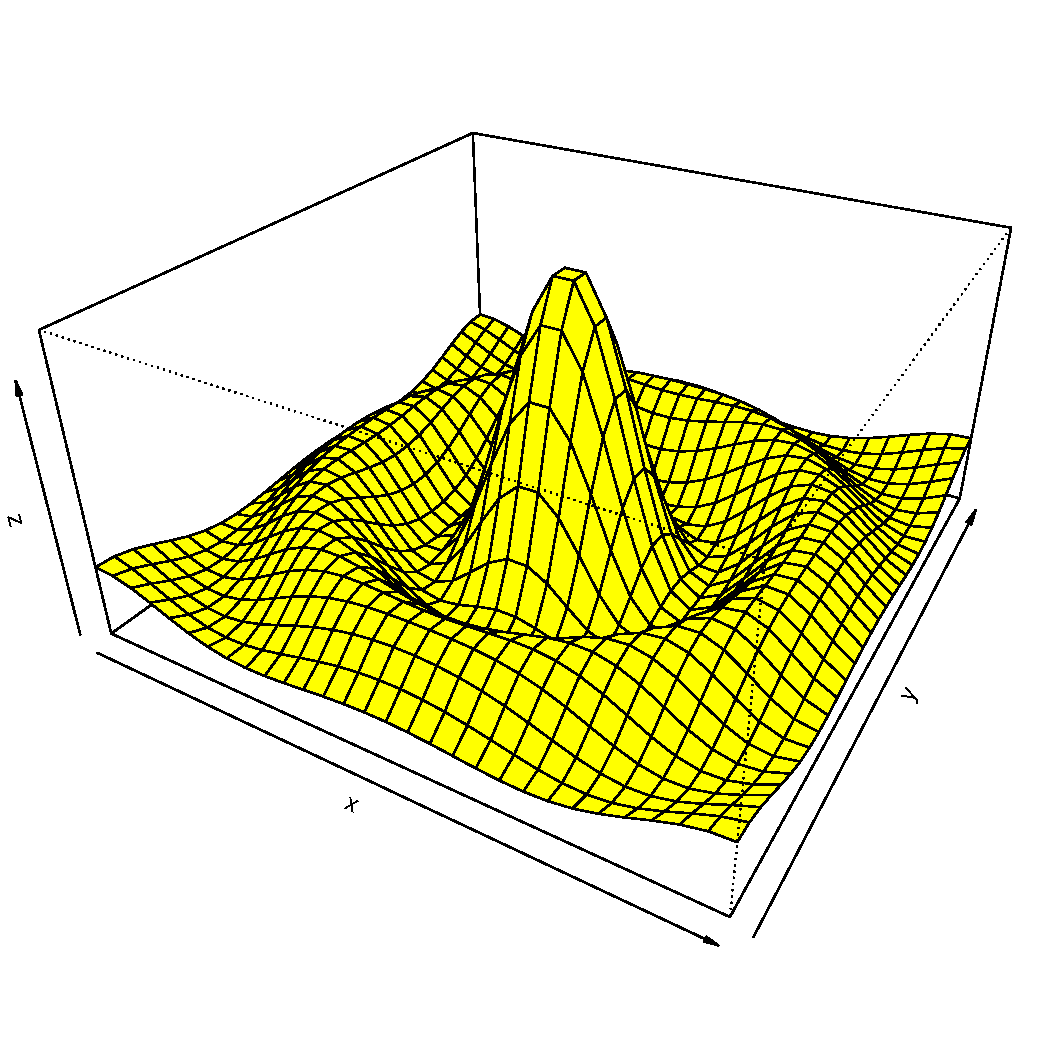
\includegraphics[height = 10cm, width = 10cm]{figure/standalone_1}
  \caption{An example of Perspective Plot been drawn by \texttt{persp()}}
  	\label{figure4}
\end{center}
\end{figure}

\newpage

From the pervious example, we discovered that the Perspective Plots is formed by a finite number of "polygon", each polygons have 4 Vertices. If we can access the values for each Vertices of the polygon, then we can reproduce this polygon. If we can access all the values of Vertices of all polygons, then we can reproduce the Perspective Plot. \\

Inorder to emulate this plot, we need to access the some information from the graphics engine display list. However, the value of the vertices are not in the display list, therefore the plot can not been reproduce directly. But we can access value of \emph{x}, \emph{y} and \emph{z}, therefore we have to re-do the calculation inorder to get values of all vertices. The folowing codes show that the value of \emph{x}, \emph{y} and \emph{z} which inputted by the user can been "catched" from the display list.

\begin{Schunk}
\begin{Sinput}
> reco = recordPlot()
> info = reco[[1]][[3]][[2]]
> ## print the values of x
> head(info[[2]])
\end{Sinput}
\begin{Soutput}
[1] -10.000000  -9.310345  -8.620690  -7.931034  -7.241379  -6.551724
\end{Soutput}
\begin{Sinput}
> ## print the values of y
> head(info[[3]])
\end{Sinput}
\begin{Soutput}
[1] -10.000000  -9.310345  -8.620690  -7.931034  -7.241379  -6.551724
\end{Soutput}
\begin{Sinput}
> ## print the values of z
> info[[4]][1:6, 1:2]
\end{Sinput}
\begin{Soutput}
           [,1]       [,2]
[1,]  0.7070981  0.6512071
[2,]  0.6512071  0.4291166
[3,]  0.4502042  0.0960367
[4,]  0.1532827 -0.2695253
[5,] -0.1766027 -0.5910827
[6,] -0.4800328 -0.8127730
\end{Soutput}
\end{Schunk}



\subsection{The translation from 3-dimension points into 2-dimension points}
The values of \emph{x}, \emph{y} and \emph{z} can been recored from the display list, which been explained by the pervious section, the next task is to use this information to reproduce the vertics in 3-dimensions.\\

As we know, the matrix, \emph{z} is computed by a specific functions, given two inputs, \emph{x} and \emph{y}, or the expression of z can been written as: $z = f(x,y)$, it contains all the values for all combination of \empth{x} and \emph{y} and the dimenstion of \empth{z} is $dim(x) \times dim(y)$.\\

\begin{Schunk}
\begin{Sinput}
> xTmp = rep(x, length(y))
> yTmp = rep(y,each = length(x))
> zTmp = as.numeric(z)
> length(xTmp) == length(zTmp) & length(yTmp) == length(zTmp)
\end{Sinput}
\begin{Soutput}
[1] TRUE
\end{Soutput}
\end{Schunk}

One 3-dimenstions points contains a set values of $(x, y, z)$, but \empth{z} is $dim(x) \times dim(y)$ matrix, x is a vector which has length of $length(x)$ and y is a vector which has length of $length(y)$. Inorder to produce the points, the dimension of \emph{x}, \emph{y} and \emph{z} need to be matched and also in a right order.\\

First step is the reduce the \emph{z} $dim(x) \times dim(y)$ matrix into a one dimension vector which has length of $dim(x) \times dim(y)$. It can been reduced by either along x direction or y direction. In this paper, we reduced along the x direction. The second step is repeat the vector x and y until the same length of z. Since z is reduced along the x direction say $z_p$, hence we repeat x until the length of y say $x_p$, and we repeat each y by the length of x, say $y_p$. At last, the combination of $x_p$, $y_p$, $z_p$ is the 3-dimensions points which preper for computing the vertics. \\

The idea of transform the points into vertics is repeating the points in a right order. From pervious section, we explained that the Perspective Plots is made by finite number of polygons. Each polygons have 4 vertics. The total number of polygons are required to be drawn is depent on the length of input \emph{x} and the length of input \emph{y}, that is, $total = (length(x) - 1) \times (length(y) - 1)$. The polygons been drawn by connecting 4 points in a specific order. The algorithm of the drawing as follows: starting from bottom-left, first connect bottom-left to bottom-right, second connect from bottom-rigth to top-right, lastly, connect top-right to top-left. Every polygons are been drawn in this order. The surface of Perspective Plots is been formed until all the polygons are been drawn. 


 
Before drawing the surface, the transformation of 3-dimensions vertics into 2-dimension vertics is required. This transformation required two main variables, the 3-dimension vertics and $4 \times 4$ viewing tranformation matrix $p$. The 3-dimenstion vertics are computed, the matrix \emph{p} can been recored from the \texttt{persp()} call. This transformation can be done easily on R by using the \texttt{trans3d()} function.

\begin{Schunk}
\begin{Sinput}
> points3d = trans3d(xTmp, yTmp, zTmp, trans)
> head(points3d$x)
\end{Sinput}
\begin{Soutput}
[1] -0.3855721 -0.3715974 -0.3567724 -0.3413650 -0.3256723 -0.3099360
\end{Soutput}
\begin{Sinput}
> head(points3d$y)
\end{Sinput}
\begin{Soutput}
[1] -0.1141316 -0.1210975 -0.1310004 -0.1428878 -0.1555315 -0.1677817
\end{Soutput}
\end{Schunk}

Because of we are drawing a 3-dimension surface in a 2-dimension plane, some polygons that stay 'behind' can not been seen, It is necessary to draw the polygons in a right order. The order defined by using the \emph{x} and \emph{y} coordinate of the 3-d vertics (but ignore the \emph{z} coordinate) combinding an other column \textbf{1}, then do the matrix multification with the viewing transformation \emph{p}. The fourth column from this multification is the drawing order of the polygons.
\begin{Schunk}
\begin{Sinput}
> orderTemp = cbind(xTmp, yTmp, 0, 1) %*% trans 
> zdepth = orderTemp[, 4]
> ## the zdepth of a set of 4 points of each polygon
> a = order(zdepth, decreasing = TRUE)
> head(a)
\end{Sinput}
\begin{Soutput}
[1] 871 872 841 873 842 874
\end{Soutput}
\end{Schunk}

\begin{Schunk}
\begin{Sinput}
> graphics:::plot(points3d$x, points3d$y, type = 'l', lty = '1212', asp = 1, axes = FALSE, xlab = '', ylab = '')
\end{Sinput}
\end{Schunk}

\end{document}
